\documentclass[
11pt, % The default document font size, options: 10pt, 11pt, 12pt
%codirector, % Uncomment to add a codirector to the title page
]{charter} 


% El títulos de la memoria, se usa en la carátula y se puede usar el cualquier lugar del documento con el comando \ttitle
\titulo{Sistema de dosificación controlada y autoajustable de líquidos aplicado a procesos industriales} 

% Nombre del posgrado, se usa en la carátula y se puede usar el cualquier lugar del documento con el comando \degreename
\posgrado{Carrera de Especialización en Sistemas Embebidos} 
%\posgrado{Carrera de Especialización en Internet de las Cosas} 
%\posgrado{Carrera de Especialización en Inteligencia Artificial}
%\posgrado{Maestría en Sistemas Embebidos} 
%\posgrado{Maestría en Internet de las cosas}
% IMPORTANTE: no omitir titulaciones ni tildación en los nombres, también se recomienda escribir los nombres completos (tal cual los tienen en su documento)
% Tu nombre, se puede usar el cualquier lugar del documento con el comando \authorname
\autor{Ing. Federico Leonardo Alderisi}

% El nombre del director y co-director, se puede usar el cualquier lugar del documento con el comando \supname y \cosupname y \pertesupname y \pertecosupname
\director{Título y Nombre del director}
\pertenenciaDirector{pertenencia} 
\codirector{} % para que aparezca en la portada se debe descomentar la opción codirector en los parámetros de documentclass -> {} %Título y Nombre del codirector
\pertenenciaCoDirector{FIUBA}

% Nombre del cliente, quien va a aprobar los resultados del proyecto, se puede usar con el comando \clientename y \empclientename
\cliente{Ing. Carmelo Alderisi}
\empresaCliente{-}
 
\fechaINICIO{23 de abril de 2024}		%Fecha de inicio de la cursada de GdP \fechaInicioName
\fechaFINALPlan{11 de junio de 2024} 	%Fecha de final de cursada de GdP
\fechaFINALTrabajo{15 de mayo de 2024}	%Fecha de defensa pública del trabajo final


\begin{document}

\maketitle
\thispagestyle{empty}
\pagebreak


\thispagestyle{empty}
{\setlength{\parskip}{0pt}
\tableofcontents{}
}
\pagebreak


\section*{Registros de cambios}
\label{sec:registro}


\begin{table}[ht]
\label{tab:registro}
\centering
\begin{tabularx}{\linewidth}{@{}|c|X|c|@{}}
\hline
\rowcolor[HTML]{C0C0C0} 
Revisión & \multicolumn{1}{c|}{\cellcolor[HTML]{C0C0C0}Detalles de los cambios realizados} & Fecha      \\ \hline
0      & Creación del documento                                 &\fechaInicioName \\ \hline
1      & Se completa hasta el punto 5 inclusive                & {6} de {mayo} de 2024 \\ \hline
%2      & Se completa hasta el punto 9 inclusive
%		  Se puede agregar algo más \newline
%		  En distintas líneas \newline
%		  Así                                                    & {día} de {mes} de 202X \\ \hline
%3      & Se completa hasta el punto 12 inclusive                & {día} de {mes} de 202X \\ \hline
%4      & Se completa el plan	                                 & {día} de {mes} de 202X \\ \hline

% Si hay más correcciones pasada la versión 4 también se deben especificar acá

\end{tabularx}
\end{table}

\pagebreak



\section*{Acta de constitución del proyecto}
\label{sec:acta}

\begin{flushright}
Buenos Aires, \fechaInicioName
\end{flushright}

\vspace{2cm}

Por medio de la presente se acuerda con el \authorname\hspace{1px} que su Trabajo Final de la \degreename\hspace{1px} se titulará ``\ttitle'' y consistirá en la implementación de un prototipo de un sistema de control de dosificación de líquidos industriales, de forma controlada y autoajustable, mediante un parámetro externo provisto por el usuario. El trabajo tendrá un presupuesto preliminar estimado de \textcolor{red}{600} horas y un costo estimado de \textcolor{red}{\$ XXX}, con fecha de inicio el \fechaInicioName\hspace{1px} y fecha de presentación pública el \textcolor{red}{fecha de presentación pública a definir}.

Se adjunta a esta acta la planificación inicial.

\vfill

% Esta parte se construye sola con la información que hayan cargado en el preámbulo del documento y no debe modificarla
\begin{table}[ht]
\centering
\begin{tabular}{ccc}
\begin{tabular}[c]{@{}c@{}}Dr. Ing. Ariel Lutenberg \\ Director posgrado FIUBA\end{tabular} & \hspace{2cm} & \begin{tabular}[c]{@{}c@{}}\clientename \\ \empclientename \end{tabular} \vspace{2.5cm} \\ 
\multicolumn{3}{c}{\begin{tabular}[c]{@{}c@{}} \supname \\ Director del Trabajo Final\end{tabular}} \vspace{2.5cm} \\
\end{tabular}
\end{table}




\section{1. Descripción técnica-conceptual del proyecto a realizar}
\label{sec:descripcion}

Un dosificador de líquidos, utilizado en procesos industriales, facilita el control de las dosis aplicadas de manera controlada, continua y precisa durante un proceso específico. Generalmente, estos sistemas incorporan un medio de bombeo que permite un flujo de líquido hacia la salida del dosificador y un caudalímetro para el sensado del caudal.

Comúnmente, los sistemas de dosificación controlada constan de un único parámetro de referencia, llamado punto de trabajo. Su valor es ingresado por el usuario y representa la dosis o caudal que se desea mantener de forma continua a la salida del dosificador. El lazo cerrado del control del sistema se ajusta a través de un circuito que adquiere la señal del caudalímetro, la compara con la del punto de trabajo ingresado por el usuario y ajusta la salida para lograrlo.

A continuación, en la figura \ref{fig:diagCaudalimetroGenerico} se ilustra un sistema dosificador continuo y controlado utilizado en la industria actualmente.

\begin{figure}[htpb]
\centering 
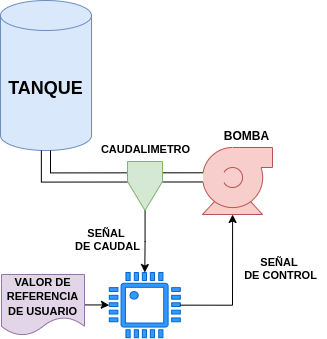
\includegraphics[width=.45\textwidth]{./Figuras/diagCaudalimetroGenerico.png}
\caption{Dosificador genérico.}
\label{fig:diagCaudalimetroGenerico}
\end{figure}

A pesar de ser un sistema utilizado en distintos procesos industriales, los sistemas de dosificación actuales no pueden transportarse ya que están fijos en una etapa del proceso. Además, estos controlan grandes o medianos caudales y su punto de trabajo se mantiene constante. En consecuencia, aquellas aplicaciones que requieran transportar un dosificador a distintos lugares o utilizar un parámetro de referencia variable para la dosificación, no pueden llevarse a cabo.

A raíz de esta problemática, se decide realizar un prototipo de un nuevo sistema de dosificación portable e innovador. A este sistema de dosificación controlada se le añade, como característica principal, la posibilidad de que el parámetro de referencia sea autoajustable, a través de un parámetro variable, en vez de uno estático como es el caso de los sistemas actuales. Además, se incorporará una interfaz de usuario que permita la interacción y configuración del sistema, como el parámetro de referencia variable, visualización de estadísticas y otras funcionalidades a definir. 

También, se utilizarán distintos subsistemas de control y alarma para el nivel del líquido del tanque, medición de temperatura y control del sistema eléctrico de alimentación. Como enfoque principal de aplicación, se desarrollará un sistema de dosificación de líquidos para aplicaciones industriales de bajo caudal.

La característica de autoajustable permite la introducción de un parámetro de referencia variable, lo que facilita el autoajuste del sistema de dosificación para adaptar el caudal de salida a las condiciones cambiantes del proceso. Esto es importante, ya que distintos procesos industriales requieren ajustes de caudal constantes. El éxito de estos procesos depende de variar el caudal en función de la magnitud de ciertos parámetros variables, como puede ser la temperatura, el peso y otros.

A continuación, en la figura \ref{fig:diagBloquesGeneral} se ilustra un diagrama en bloques del sistema propuesto. Se pueden observar los distintos bloques que conforman el sistema electrónico y el bloque del sistema eléctrico de alimentación que se desarrollará durante este trabajo. El sistema electromecánico no será incluido.

\begin{figure}[htpb]
\centering 
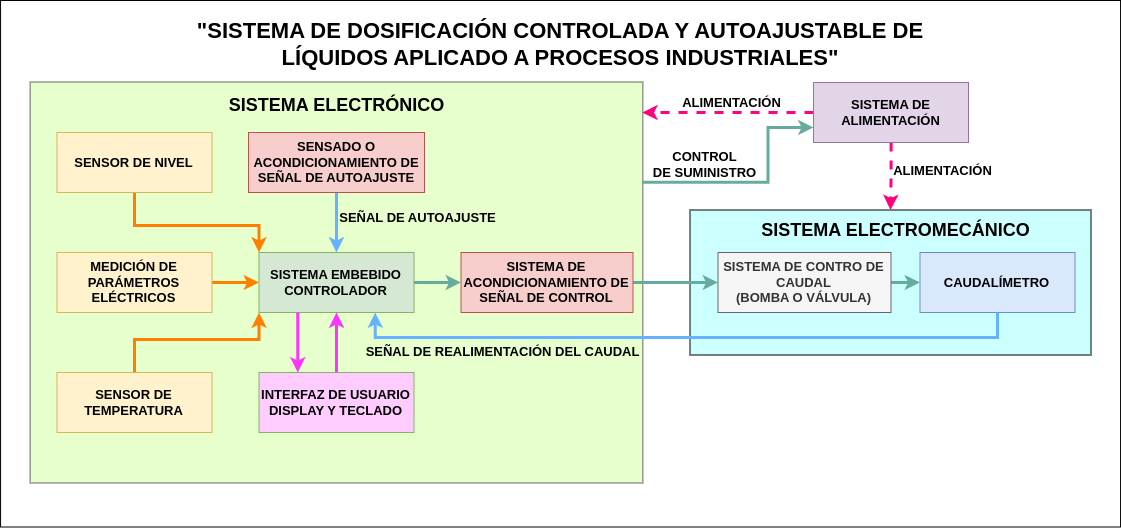
\includegraphics[width=.95\textwidth]{./Figuras/diagBloquesGeneral.png}
\caption{Diagrama en bloques del sistema.}
\label{fig:diagBloquesGeneral}
\end{figure}

Es importante destacar que este proyecto se realiza como un emprendimiento personal, junto a un colaborador, que será responsable del diseño mecánico e hidráulico. Este proyecto se circunscribe al desarrollo del firmware y hardware de este sistema.

\section{2. Identificación y análisis de los interesados}
\label{sec:interesados}


\begin{table}[ht]
%\caption{Identificación de los interesados}
%\label{tab:interesados}
\begin{tabularx}{\linewidth}{@{}|l|X|X|l|@{}}
\hline
\rowcolor[HTML]{C0C0C0} 
Rol           & Nombre y Apellido & Organización 	& Puesto 	\\ \hline
%Auspiciante   &                   &              	&        	\\ \hline
Cliente       & \clientename      &\empclientename	& Consultor comercial	\\ \hline
%Impulsor      &                   &              	&        	\\ \hline
Responsable   & \authorname       & FIUBA        	& Alumno 	\\ \hline
Colaboradores & Ing. Julián Marchese                  & -              	& Diseñador       	\\ \hline
Orientador    & \supname	      & \pertesupname 	& Director del Trabajo Final \\ \hline
%Equipo        & miembro1 \newline 
%				miembro2          &              	&        	\\ \hline
%Opositores    &                   &              	&        	\\ \hline
%Usuario final &                   &              	&        	\\ \hline
\end{tabularx}
\end{table}

Las características principales de cada uno de los interesados listados previamente son:

\begin{itemize}
	\item Cliente: ingeniero agrónomo de amplia experiencia en la industria alimentaria, agropecuaria y en el área comercial. Es una persona rigurosa y exigente al observar posibles mejoras en procesos industriales. Busca agilizar y eficientizar procedimientos y mecanismos agrícolas. La amplia experiencia permite que se pueda disponer de información respecto a los diferentes campos de aplicación del sistema a desarrollar, como así también los requerimientos mínimos a cumplir. 
	\item Colaborador: ingeniero electromecánico que trabaja como diseñador y desarrollador de sistemas mecánicos, térmicos e hidráulicos. Una persona que trabaja de forma profesional, que al desarrollar proyectos busca de forma exhaustiva cumplir con sus objetivos. Consta de un amplio conocimiento en maquinarias agropecuarias de siembra y cosecha, en los que puede ser aplicado el sistema a desarrollar.
	\item Orientador: \textcolor{red}{A DEFINIR}.
\end{itemize}


\section{3. Propósito del proyecto}
\label{sec:proposito}

Se propone el desarrollo de un sistema prototipo de dosificación controlada y continua para líquidos en aplicaciones industriales. Este sistema permitirá autoajustarse en función de un parámetro externo dinámico o un parámetro estático ingresado por el usuario. Dado su enfoque en dosificación de bajo caudal, se diseñará para ser fácilmente transportable y con dimensiones adecuadas para ser manipulado por una persona. Este sistema constará de varios subsistemas, incluyendo una interfaz de usuario para el ingreso de parámetros de control y visualización, control de parámetros ambientales y eléctricos, así como control de nivel de tanque, entre otros.

La implementación de este sistema resuelve la problemática actual relacionada con la dificultad para mantener un flujo de dosificación autoajustable. Los sistemas de bajo costo disponibles en la actualidad no incorporan esta característica y carecen de portabilidad. Por lo tanto, el objetivo de este desarrollo es ofrecer una solución robusta, confiable y segura para su uso industrial. Esto permitirá a los usuarios reemplazar los antiguos procedimientos de dosificación aproximada en sus procesos industriales.

\section{4. Alcance del proyecto}
\label{sec:alcance}

Como se especificó en la sección \ref{sec:descripcion}, el prototipo del sistema de dosificador controlada y autoajustable consta de distintas características. Estas determinan el alcance de este trabajo final correspondiente a la  \degreename\hspace{1px}.

Este proyecto incluye:

\begin{itemize}
	\item Desarrollo del prototipo funcional del sistema de dosificación controlada y autoajustable, consta de:
			\begin{itemize}
	\item Definición del algoritmo de control para la dosificación de líquidos.
	\item Desarrollo del sistema de acondicionamiento señales de control y señales de realimentación.
	\item Implementación del algoritmo de control en un sistema embebido.
	\item Diseño e implementación de una interfaz de usuario para controlar y visualizar el funcionamiento del sistema.
	\item Adquisición de parámetros ambientales y eléctricos requeridos.
	\item Determinar un sistema de alimentación acorde al uso.
			\end{itemize}
	\item Pruebas funcionales y de concepto.
	\item Reporte de resultados.
\end{itemize}

Este proyecto no incluye:

\begin{itemize}
	\item Desarrollo del sistema hidráulico y mecánico.
	\item Construcción de un producto final comercial.
	\item Certificación del sistema a través de estándares.
\end{itemize}


\section{5. Supuestos del proyecto}
\label{sec:supuestos}

Para el desarrollo del presente proyecto se tiene a consideración los siguientes supuestos:

\begin{itemize}
	\item Interés del mercado y del cliente: actualmente, no existen sistemas de estas características que se puedan comparar con lo propuesto. En consecuencia, el cliente tiene interés en que se desarrolle este sistema.
	\item Disponibilidad de materiales: a pesar de que es complicado el proceso de importar productos electrónicos, es viable en este caso, ya que no se necesitan grandes cantidades para realizar un primer prototipo.
	\item Desarrollo del prototipo: este sistema solo será fabricado a nivel de prototipo, sin realizar iteraciones en su diseño.
	\item Presupuesto: este proyecto tendrá los fondos disponibles para financiar los gastos de inversión inicial y desarrollo.
	\item Tiempo: se dispondrá del tiempo establecido por la planificación para lograr los objetivos.
\end{itemize}


\section{6. Requerimientos}
\label{sec:requerimientos}

\begin{enumerate}
	\item Requerimientos funcionales:
		\begin{enumerate}
			\item Control:
			\begin{enumerate}
			\item El prototipo debe permitir controlar el caudal de líquido dosificado en milímetros cúbicos por minuto.
			\item La muestra de caudal debe poder ser adquirida desde una señal provista por un caudalímetro.
			\item La señal de salida del sistema de control debe permitir ser aplicada sobre un dispositivo de accionamiento, como una bomba o válvula, a definir durante el desarrollo.
			\item El sistema de control debe permitir que el usuario ingrese un valor como punto de trabajo o admitir un valor de referencia externo que funcione como punto de trabajo variable.
			\item El sistema debe permitir dosificar en forma continua, teniendo en cuenta el nivel del líquido del tanque y los límites de dosificación (de trescientos a \textcolor{red}{A DEFINIR} milímetros cúbicos por minuto).
			\item El sistema debe lograr el equilibrio en un tiempo acotado, en función del proceso en el que se utilizará, siendo este tiempo menor a 3 segundos.			
			\item El valor de referencia externo debe ser un valor acondicionado, que provenga de una entrada del sistema embebido utilizado.
			\item El sistema de alimentación debe ser monitoreado para mantener la integridad del dosificador.
			\item Otros parámetros a definir, como temperatura o variables del sistemas, deben poder ser monitoreados.
			\end{enumerate}
			\item Interfaz de usuario:
			\begin{enumerate}
			\item La interfaz debe permitir configurar la dosis y cambiar el modo de funcionamiento.
			\item La pantalla debe presentar el estado general del dosificador, su modo de funcionamiento, las estadísticas, configuraciones y posibles alarmas a definir.
			\item El teclado debe permitir ingresar el valor de dosificación de forma numérica, además de incluir las funciones para cambiar de menú, encender y apagar la bomba, y navegar dentro del menú.
			\item El prototipo debe mostrar señales lumínicas en función del estado de la alimentación, modo de funcionamiento y alarmas.
			\end{enumerate}
			\item Alimentación:
			\begin{enumerate}
			\item El sistema de alimentación debe poder ser conectado a una línea de alimentación de 12 Volts C.C. y adaptar esta tensión a lo requerido por el dosificador.
			\item El usuario debe poder encender o apagar el sistema de alimentación y, en consecuencia, el dosificador.
			\item El controlador debe poder apagar el sistema de alimentación, como así también limitar y aislar los puntos de falla, como el sistema de accionamiento a definir.
			\end{enumerate}
		\end{enumerate}
		
	\item Requerimientos de documentación:
		\begin{enumerate}
			\item Se debe documentar de manera clara las instrucciones de uso del dosificador.
			\item El sistema de control, junto a sus entradas y salidas, deben ser especificados eléctricamente para realizar su posterior conexión.
			\item Se debe documentar las conexiones de alimentación y del sistema electromecánico para su puesta en marcha.
		\end{enumerate}
		
	\item Requerimiento de testing y pruebas:
		\begin{enumerate}
			\item Se deben presentar resultados de las pruebas unitarias a definir y de integración.
			\item Se deben realizar pruebas de aceptación en presencia del cliente.
			\item Las pruebas del sistema deben evidenciar los objetivos propuestos en este trabajo.
		\end{enumerate}
		
	\item Requerimientos de comunicación (opcional): el desarrollador podría proponer un sistema de comunicación inalámbrico, que permita al usuario conectarse a través de un celular y pueda configurar y visualizar datos.
\end{enumerate}

\section{7. Historias de usuarios (\textit{Product backlog})}
\label{sec:backlog}

En esta sección se describen las historias de usuarios y sus puntajes correspondientes. Los 3 aspectos que definirán los puntajes de las historias son los siguientes:

\begin{enumerate}
\item Dificultad: cantidad del trabajo a realizar.
\item Complejidad: complejidad del trabajo a realizar.
\item Incertidumbre: riesgo del trabajo a realizar.
\end{enumerate}

Se utilizará una escala de 3 puntos, donde el valor más alto implica mayor costo. A continuación, se listan los puntajes para cada item dentro de los \textit{Story points}.

\begin{enumerate}
\item Dificultad:
\begin{itemize}
	\item Baja: 1.
	\item Media: 2.
	\item Alta: 3.
\end{itemize}
\item Complejidad:
\begin{itemize}
	\item Baja: 1.
	\item Media: 2.
	\item Alta: 3.
\end{itemize}
\item Incertidumbre:
\begin{itemize}
	\item Baja: 1.
	\item Media: 2.
	\item Alta: 3.
\end{itemize}
\end{enumerate}

Historia de usuarios:

\begin{enumerate}
\item Operario: ``Como operario de la industria química, desearía un dosificador que permita cambiar la dosificación de forma automática para no tener que hacerlo manualmente."

\begin{itemize}
	\item Dificultad media (2): realizar un sistema de control automático que depende de un parámetro variable es algo que puede generar inestabilidades durante su control. A pesar de esto, si se definen los tiempos de accionamiento y los límites, se puede realizar.
	\item Complejidad alta (3): requiere implementar un sistema de control digital, donde se controle y limite la variable de entrada y salida, para evitar oscilaciones. Si el parámetro de entrada oscila rápidamente, puede generar inestabilidades durante la dosificación, por lo que es algo que se debe caracterizar.
	\item Riesgo medio (2): en caso de que no pueda aplicarse un control automático en todos los casos, el sistema permite igualmente ingresar por teclado el punto de trabajo deseado, por lo que el usuario podrá de todas maneras reemplazar el sistema manual que utiliza actualmente.
\end{itemize}

\textit{Story points}: 7.

\item Ingeniero agrónomo: ``Durante la siembra, se inyectan productos agropecuarios a la tierra y los operarios deben cambiar manualmente la dosis. Esto cuesta mucho durante el proceso ya que no es algo que se pueda hacer rápidamente, además de que no se puede controlar a simple vista. Desearía un sistema que permita ingresar un valor de dosis por teclado rápidamente y que sea visible, para constatar que este es el correcto y así evitar errores de dosificación."

\begin{itemize}
	\item Dificultad baja (1): realizar una interfaz de usuario a través de un teclado y una pantalla no es algo que requiera grandes esfuerzos.
	\item Complejidad media (2): este sistema debe ser robusto y confiable, por lo que la validación de datos, confirmación y ajustes de parámetros es indispensable. Además, se debe proveer una interfaz duradera, ya que será utilizada en el campo.
	\item Riesgo bajo (1): para lograr este objetivo, se debe analizar productos con interfaz de usuario que se utilizan en el campo. De esta manera se puede obtener una idea de qué tipo de interfaz rápida y confiable se puede utilizar. A pesar de esto, una mala interfaz puede generar molestia al momento de utilizar el dosificador.
\end{itemize}

\textit{Story points}: 4


\end{enumerate}


\section{8. Entregables principales del proyecto}
\label{sec:entregables}


Los entregables del proyecto son:

\begin{itemize}
	\item Un prototipo.
	\item Manual de usuario.
	\item Instrucciones de puesta en marcha, que incluye las especificaciones de las distintas conexiones eléctricas.
	\item Diagrama de circuitos esquemáticos.
	\item Memoria del trabajo final.
\end{itemize}


\section{9. Desglose del trabajo en tareas}
\label{sec:wbs}

A continuación, se desglosa el trabajo en tareas con su duración estimada:

\begin{enumerate}
\item Desarrollo del prototipo (395 h).

	\begin{enumerate}
	\item Modularización del sistema y definición de funcionalidades (80 h).
	
		\begin{enumerate}
		\item Selección del dispositivo de accionamiento, medición de caudal y caracterización de las señales correspondientes (20 h).
		\item Definición del sistema de control y algoritmo (30 h).
		\item Determinación los periféricos de entrada y salida (15 h).
		\item Definición de circuitos e interfaces de acondicionamiento de señales (15 h).
		\end{enumerate}
		
	\item Selección del sistema embebido, circuitos periféricos e implementación del programa (160 h).
	
		\begin{enumerate}
		\item Selección del sistema embebido, acorde a los requerimientos y el análisis previo (15 h).
		\item Programación del sistema de control principal (40 h).
		\item Programación de drivers (40 h).
		\item Programación de la interfaz de usuario (35 h).
		\item Programación de sistemas secundarios (30 h).
		\end{enumerate}

		
	\item Hardware, sistema de alimentación, circuitos periféricos e interfaces de conexión (155 h).
	
		\begin{enumerate}
		\item Definición de dispositivos y periféricos generales (interfaz de usuario, adaptadores de señales y otros) (30 h).
		\item Diseño del sistema de alimentación (15 h).
		\item Dimensionamiento de componentes (15 h).
		\item Diseño de esquemáticos (35 h).
		\item Diseño de placas y conexionado (30 h).
		\item Ensamblaje del prototipo (20 h).
		\item Pruebas eléctricas e inspección general (10 h).
		\end{enumerate}		
		
	\end{enumerate}		
		
\item Testing (95 h).
	
	\begin{enumerate}
	\item Realizar pruebas unitarias (40 h).
	\item Realizar pruebas de integración (35 h).
	\item Realizar pruebas del sistema (20 h).
	\end{enumerate}		
		
		
\item Documentación (125 h).

	\begin{enumerate}
	\item Desarrollo de reporte de testing (25 h).
	\item Elaboración del manual e instrucciones (20 h).
	\item Redacción del informe de avance (20 h).
	\item Redacción de la memoria del trabajo final (40 h).
	\item Elaboración de la presentación del proyecto (20 h).
	\end{enumerate}

\end{enumerate}

Total de horas estimadas: 615 h.

\section{10. Diagrama de Activity On Node}
\label{sec:AoN}

\begin{consigna}{red}
Armar el AoN a partir del WBS definido en la etapa anterior.

Una herramienta simple para desarrollar los diagramas es el Draw.io (\url{https://app.diagrams.net/}).
\href{https://app.diagrams.net}{Draw.io}


\begin{figure}[htpb]
\centering 
\includegraphics[width=.8\textwidth]{./Figuras/AoN.png}
\caption{Diagrama de \textit{Activity on Node}.}
\label{fig:AoN}
\end{figure}

Indicar claramente en qué unidades están expresados los tiempos.
De ser necesario indicar los caminos semi críticos y analizar sus tiempos mediante un cuadro.
Es recomendable usar colores y un cuadro indicativo describiendo qué representa cada color.

\end{consigna}

\section{11. Diagrama de Gantt}
\label{sec:gantt}

\begin{consigna}{red}
Existen muchos programas y recursos \textit{online} para hacer diagramas de Gantt, entre los cuales destacamos:

\begin{itemize}
\item Planner
\item GanttProject
\item Trello + \textit{plugins}. En el siguiente link hay un tutorial oficial: \\ \url{https://blog.trello.com/es/diagrama-de-gantt-de-un-proyecto}
\item Creately, herramienta online colaborativa. \\\url{https://creately.com/diagram/example/ieb3p3ml/LaTeX}
\item Se puede hacer en latex con el paquete \textit{pgfgantt}\\ \url{http://ctan.dcc.uchile.cl/graphics/pgf/contrib/pgfgantt/pgfgantt.pdf}
\end{itemize}

Pegar acá una captura de pantalla del diagrama de Gantt, cuidando que la letra sea suficientemente grande como para ser legible. 
Si el diagrama queda demasiado ancho, se puede pegar primero la ``tabla'' del Gantt y luego pegar la parte del diagrama de barras del diagrama de Gantt.

Configurar el software para que en la parte de la tabla muestre los códigos del EDT (WBS).\\
Configurar el software para que al lado de cada barra muestre el nombre de cada tarea.\\
Revisar que la fecha de finalización coincida con lo indicado en el Acta Constitutiva.

En la figura \ref{fig:gantt}, se muestra un ejemplo de diagrama de gantt realizado con el paquete de \textit{pgfgantt}. 
En la plantilla pueden ver el código que lo genera y usarlo de base para construir el propio.

Las fechas pueden ser calculadas utilizando alguna de las herramientas antes citadas. Sin embargo, el siguiente ejemplo
fue elaborado utilizando 
\href{https://docs.google.com/spreadsheets/d/1fBz8NhSpc4tkkhz3KjJCbh1nR_ltDkfEcZi4tZXduqs}{esta hoja de cálculo}.

Es importante destacar que el ancho del diagrama estará dado por la longitud del texto utilizado para las tareas 
(Ejemplo: tarea 1, tarea 2, etcétera) y el valor \textit{x unit}. Para mejorar la apariencia del diagrama, es necesario
ajustar este valor y, quizás, acortar los nombres de las tareas.

\begin{figure}[htpb]
  \begin{center}
    \begin{ganttchart}[
      time slot unit=day,
      time slot format=isodate,
      x unit=0.038cm,
      y unit title=0.7cm,
      y unit chart=0.6cm,
      milestone/.append style={xscale=4}
      ]{2021-03-05}{2021-12-16}
      \gantttitlecalendar*{2021-03-05}{2021-12-16}{year} \\
      \gantttitlecalendar*{2021-03-05}{2021-12-16}{month} \\
      \ganttgroup{Duración Total}{2021-03-05}{2021-12-16} \\
      %%%%%%%%%%%%%%%%%Organización
      \ganttgroup{Organización}{2021-03-05}{2021-04-16} \\
      \ganttbar{Planificación del proyecto}{2021-03-05}{2021-04-15} \\
      %%%%%%%%%%%%%%%%%Ejecución
      \ganttgroup{Ejecución}{2021-04-16}{2021-10-21} \\
      \ganttbar{Tarea 1}{2021-04-16}{2021-04-29} \\
      \ganttbar{Tarea 2}{2021-04-30}{2021-05-13} \\
      \ganttbar{Tarea 3}{2021-05-14}{2021-05-27} \\
      \ganttbar{Tarea 4}{2021-05-28}{2021-07-12} \\
      \ganttbar{Tarea 5}{2021-07-13}{2021-08-09} \\
      \ganttbar{Tarea 6}{2021-08-10}{2021-09-23} \\
      \ganttbar{Tarea 7}{2021-09-24}{2021-09-30} \\
      \ganttbar{Tarea 8}{2021-10-01}{2021-10-14} \\
      \ganttbar{Tarea 9}{2021-10-15}{2021-10-21} \\
      % %%%%%%%%%%%%%%%%%Finalización
      \ganttgroup{Finalización}{2021-10-22}{2021-12-16} \\
      \ganttbar{Memoria v1}{2021-10-22}{2021-11-04} \\
      \ganttbar{Memoria v2}{2021-11-05}{2021-11-18} \\
      \ganttbar{Memoria final}{2021-11-19}{2021-12-02} \\
      % La fecha del siguiente milestone es la fecha en que terminamos la memoria
      \ganttmilestone{Enviar memoria al director}{2021-12-02} \\
      \ganttbar{Elaborar la presentación}{2021-12-03}{2021-12-16} \\
      \ganttmilestone{Ensayo de la presentación}{2021-12-16} \\
      %%%%%%%%%%%%%%%%%%%%%%%%%%%%%%%%%%%%%%%%%%%%%%%%%%%%%%%%%%%%%%%
    \end{ganttchart}
  \end{center}
  \caption{Diagrama de gantt de ejemplo}
  \label{fig:gantt}
\end{figure}


\begin{landscape}
\begin{figure}[htpb]
\centering 
\includegraphics[height=.85\textheight]{./Figuras/Gantt-2.png}
\caption{Ejemplo de diagrama de Gantt (apaisado).} %Modificar este título acorde.
\label{fig:diagGantt}
\end{figure}

\end{landscape}

\end{consigna}


\section{12. Presupuesto detallado del proyecto}
\label{sec:presupuesto}

\begin{consigna}{red}
Si el proyecto es complejo entonces separarlo en partes:
\begin{itemize}
	\item Un total global, indicando el subtotal acumulado por cada una de las áreas.
	\item El desglose detallado del subtotal de cada una de las áreas.
\end{itemize}

IMPORTANTE: No olvidarse de considerar los COSTOS INDIRECTOS.

Incluir la aclaración de si se emplea como moneda el peso argentino (ARS) o si se usa moneda extranjera (USD, EUR, etc). Si es en moneda extranjera se debe indicar la tasa de conversión respecto a la moneda local en una fecha dada.

\end{consigna}

\begin{table}[htpb]
\centering
\begin{tabularx}{\linewidth}{@{}|X|c|r|r|@{}}
\hline
\rowcolor[HTML]{C0C0C0} 
\multicolumn{4}{|c|}{\cellcolor[HTML]{C0C0C0}COSTOS DIRECTOS} \\ \hline
\rowcolor[HTML]{C0C0C0} 
Descripción &
  \multicolumn{1}{c|}{\cellcolor[HTML]{C0C0C0}Cantidad} &
  \multicolumn{1}{c|}{\cellcolor[HTML]{C0C0C0}Valor unitario} &
  \multicolumn{1}{c|}{\cellcolor[HTML]{C0C0C0}Valor total} \\ \hline
 &
  \multicolumn{1}{c|}{} &
  \multicolumn{1}{c|}{} &
  \multicolumn{1}{c|}{} \\ \hline
 &
  \multicolumn{1}{c|}{} &
  \multicolumn{1}{c|}{} &
  \multicolumn{1}{c|}{} \\ \hline
\multicolumn{1}{|l|}{} &
   &
   &
   \\ \hline
\multicolumn{1}{|l|}{} &
   &
   &
   \\ \hline
\multicolumn{3}{|c|}{SUBTOTAL} &
  \multicolumn{1}{c|}{} \\ \hline
\rowcolor[HTML]{C0C0C0} 
\multicolumn{4}{|c|}{\cellcolor[HTML]{C0C0C0}COSTOS INDIRECTOS} \\ \hline
\rowcolor[HTML]{C0C0C0} 
Descripción &
  \multicolumn{1}{c|}{\cellcolor[HTML]{C0C0C0}Cantidad} &
  \multicolumn{1}{c|}{\cellcolor[HTML]{C0C0C0}Valor unitario} &
  \multicolumn{1}{c|}{\cellcolor[HTML]{C0C0C0}Valor total} \\ \hline
\multicolumn{1}{|l|}{} &
   &
   &
   \\ \hline
\multicolumn{1}{|l|}{} &
   &
   &
   \\ \hline
\multicolumn{1}{|l|}{} &
   &
   &
   \\ \hline
\multicolumn{3}{|c|}{SUBTOTAL} &
  \multicolumn{1}{c|}{} \\ \hline
\rowcolor[HTML]{C0C0C0}
\multicolumn{3}{|c|}{TOTAL} &
   \\ \hline
\end{tabularx}%
\end{table}


\section{13. Gestión de riesgos}
\label{sec:riesgos}

\begin{consigna}{red}
a) Identificación de los riesgos (al menos cinco) y estimación de sus consecuencias:
 
Riesgo 1: detallar el riesgo (riesgo es algo que si ocurre altera los planes previstos de forma negativa)
\begin{itemize}
	\item Severidad (S): mientras más severo, más alto es el número (usar números del 1 al 10).\\
	Justificar el motivo por el cual se asigna determinado número de severidad (S).
	\item Probabilidad de ocurrencia (O): mientras más probable, más alto es el número (usar del 1 al 10).\\
	Justificar el motivo por el cual se asigna determinado número de (O). 
\end{itemize}   

Riesgo 2:
\begin{itemize}
	\item Severidad (S): X.\\
	Justificación...
	\item Ocurrencia (O): Y.\\
	Justificación...
\end{itemize}

Riesgo 3:
\begin{itemize}
	\item Severidad (S):  X.\\
	Justificación...
	\item Ocurrencia (O): Y.\\
	Justificación...
\end{itemize}


b) Tabla de gestión de riesgos:      (El RPN se calcula como RPN=SxO)

\begin{table}[htpb]
\centering
\begin{tabularx}{\linewidth}{@{}|X|c|c|c|c|c|c|@{}}
\hline
\rowcolor[HTML]{C0C0C0} 
Riesgo & S & O & RPN & S* & O* & RPN* \\ \hline
       &   &   &     &    &    &      \\ \hline
       &   &   &     &    &    &      \\ \hline
       &   &   &     &    &    &      \\ \hline
       &   &   &     &    &    &      \\ \hline
       &   &   &     &    &    &      \\ \hline
\end{tabularx}%
\end{table}

Criterio adoptado: 

Se tomarán medidas de mitigación en los riesgos cuyos números de RPN sean mayores a...

Nota: los valores marcados con (*) en la tabla corresponden luego de haber aplicado la mitigación.

c) Plan de mitigación de los riesgos que originalmente excedían el RPN máximo establecido:
 
Riesgo 1: plan de mitigación (si por el RPN fuera necesario elaborar un plan de mitigación).
  Nueva asignación de S y O, con su respectiva justificación:
  \begin{itemize}
	\item Severidad (S*): mientras más severo, más alto es el número (usar números del 1 al 10).
          Justificar el motivo por el cual se asigna determinado número de severidad (S).
	\item Probabilidad de ocurrencia (O*): mientras más probable, más alto es el número (usar del 1 al 10).
          Justificar el motivo por el cual se asigna determinado número de (O).
	\end{itemize}

Riesgo 2: plan de mitigación (si por el RPN fuera necesario elaborar un plan de mitigación).
 
Riesgo 3: plan de mitigación (si por el RPN fuera necesario elaborar un plan de mitigación).

\end{consigna}


\section{14. Gestión de la calidad}
\label{sec:calidad}

\begin{consigna}{red}
Elija al menos diez requerimientos que a su criterio sean los más importantes/críticos/que aportan más valor y para cada uno de ellos indique las acciones de verificación y validación que permitan asegurar su cumplimiento.

\begin{itemize} 
\item Req \#1: copiar acá el requerimiento con su correspondiente número.

\begin{itemize}
	\item Verificación para confirmar si se cumplió con lo requerido antes de mostrar el sistema al cliente. Detallar.
	\item Validación con el cliente para confirmar que está de acuerdo en que se cumplió con lo requerido. Detallar. 
\end{itemize}

\end{itemize}

Tener en cuenta que en este contexto se pueden mencionar simulaciones, cálculos, revisión de hojas de datos, consulta con expertos, mediciones, etc.  

Las acciones de verificación suelen considerar al entregable como ``caja blanca'', es decir se conoce en profundidad su funcionamiento interno.  

En cambio, las acciones de validación suelen considerar al entregable como ``caja negra'', es decir, que no se conocen los detalles de su funcionamiento interno.

\end{consigna}

\section{15. Procesos de cierre}    
\label{sec:cierre}

\begin{consigna}{red}
Establecer las pautas de trabajo para realizar una reunión final de evaluación del proyecto, tal que contemple las siguientes actividades:

\begin{itemize}
	\item Pautas de trabajo que se seguirán para analizar si se respetó el Plan de Proyecto original:\\
	 - Indicar quién se ocupará de hacer esto y cuál será el procedimiento a aplicar. 
	\item Identificación de las técnicas y procedimientos útiles e inútiles que se emplearon, los problemas que surgieron y cómo se solucionaron:\\
	 - Indicar quién se ocupará de hacer esto y cuál será el procedimiento para dejar registro.
	\item Indicar quién organizará el acto de agradecimiento a todos los interesados, y en especial al equipo de trabajo y colaboradores:\\
	  - Indicar esto y quién financiará los gastos correspondientes.
\end{itemize}

\end{consigna}

\end{document}
